\documentclass[twoside,openright,a4paper,11pt,french]{article}
\usepackage[utf8]{inputenc}
\usepackage[french]{babel}
\usepackage[T1]{fontenc}
\usepackage{emptypage}
\usepackage{amsmath}

% Utilisation d'url
\usepackage{url}
\urlstyle{sf}

% Utilisation d'images, stockées dans le répertoire ./pics/
\usepackage{graphicx}
\graphicspath{pics/}

% Définition des marges
\usepackage{geometry}
\geometry{
  left=25mm,
  right=25mm,
  top=25mm,
  bottom=25mm,
  foot=15mm
}
\usepackage{listings}
\usepackage{color}

\definecolor{gray}{rgb}{0.8,0.8,0.8}

\begin{document}

\pagestyle{plain}
\setlength{\parindent}{0pt}
% La page de garde
\thispagestyle{empty}

\begin{center}
       \noindent
       
\includegraphics[height=2.5cm]{./pics/uds.eps}       
       
       \vfill\vfill

    {\large \textsc{Licence 3 de Sciences, mention Informatique}}

    \bigskip\bigskip

    {\large \textsc{Intelligence Artificielle}}

    \vfill\vfill

% Titre du document
    {\huge \sc
      \begin{center} 
        Rapport sur le projet: \\
        Perceptron et perceptron multi-couchers avec Neuroph
      \end{center}}

    \vfill\vfill

    {\large Présenté par}

\medskip

% Identité des auteurs
    {\large Victor \textsc{Constans}}\\
    {\large Luigi  \textsc{Coniglio}}\\
\bigskip

\end{center}



% La table des matières
\parskip=0pt
\tableofcontents


\vspace{5cm}

%Start content

\section{Fonctions booléennes}

Dans cette premiere section de ce rapport on se propose
de implementer des fonctions booléennes a l'aide des reseaux
de neurones. 

\subsection{"Et" logique}

En matematique la conjonction logique $\land$ est un
connecteur logique que, etant donne deux propositions $A$ et $B$
forme une nouvelle propositions $A \land B$ qui est vrai seulement
si $A$ et $B$ sont vraies.

\begin{table}[h]
  \centering
% On paramètre ici le placement du texte dans les cases, en mode paragraphe de 5cm de large dans la case de gauche ("p{5cm}") et automatique avec un alignement à droite dans la case de droite ('r')
  \begin{tabular}{| c | c | c |}
    \hline
    \textbf{$A$} & \textbf{$B$} & \textbf{$A \land B$}\\
    \hline
    0 & 0  & 0 \\
    \hline
    0 & 1  & 0 \\
    \hline
    1 & 0  & 0 \\
    \hline
    1 & 1  & 1 \\
    \hline
  \end{tabular}
  \caption{Table de verite de $A \land B$}
  \label{tab:et}
\end{table}




\subsection{Un perceptron pour $\land$} 

Est it possible d'utiliser un perceptron pour apprendre la fonction logique
"et"? Bien sur, en effet meme un perceptron mono couche est sufficent pour
obtenir cet resultat.\\

Le perceptron peut etre utilise comme un classifieur linéaire, cad. l'algorithme du
perceptron perment de reconnaitre et donc classifier des donnes (ou points)
linearement separables.\\

Un ensemble de points dans le plan caracterise par deux sous-classes disjointes
de points, est dit linearement separable si il existe une droite qui separe
completement les deux sous-classes.\\

Dans trois dimension un ensemble est linearement separable si il existe un plan
qui separe les deux classes. Dans quatre ou plus dimensions on ne parlera plus de
plan mais de hyperplan.


\begin{figure}[h]
\centering
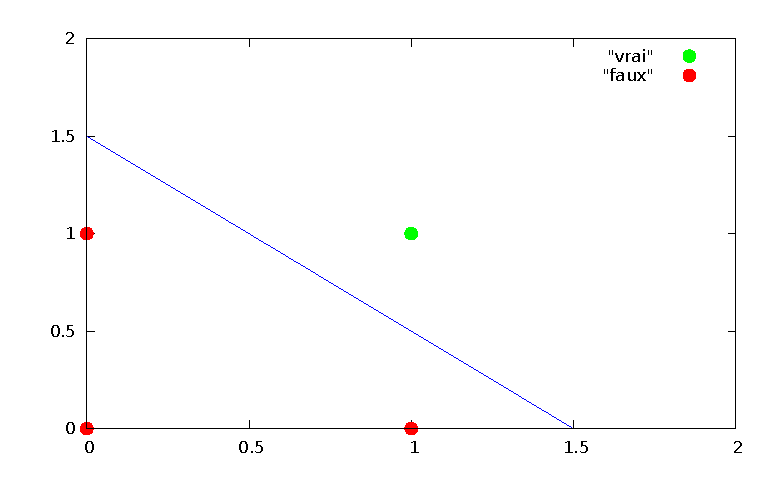
\includegraphics[width=10cm]{./pics/and/and.eps}
\caption{La fonction logique "et" est linearement separable}
\label{fig:and}
\end{figure}


Comme montre la figure \ref{fig:and} la fonction "et" est bien linearement
separable.  Etant donne que tout ensemble linéairement séparable peut être
discriminé par un perceptron on est sur de pouvoir trouver un perceptron qui
engendre la fonction booléenne $\land$.










%End content

\addcontentsline{toc}{section}{Références}
\bibliographystyle{plain}
\bibliography{rapport}

\end{document}
